\title{Dynamic Programming -- Introduction}
\author{William M Volckmann II}
\documentclass[12pt]{article}
\usepackage{bm}
\usepackage{amsmath}
\usepackage{amsfonts}
\usepackage{graphicx}
\usepackage{amssymb}
\usepackage{amsthm}
\usepackage{setspace}
\usepackage{amsthm}
\usepackage{mathtools}
\usepackage{enumitem}
\usepackage{xifthen}
\usepackage{titlesec}
\usepackage[normalem]{ulem}
\usepackage[final]{pdfpages}
%\usepackage[top=1.25in, left=1.25in, right=1.25in]{geometry}

\newcommand{\C}{\mathbb{C}}
\newcommand{\F}{\mathbb{F}}
\newcommand{\N}{\mathbb{N}}
\newcommand{\Q}{\mathbb{Q}}
\newcommand{\R}{\mathbb{R}}
\newcommand{\Z}{\mathbb{Z}}
\newcommand{\Chi}{\mathcal{X}}
\newcommand{\grad}{\nabla}
\newcommand{\B}{\beta}
\newcommand{\BH}{\hat{\beta}}
\newcommand{\bh}{\hat{\beta}}
\newcommand{\sumn}{\sum_{i=1}^n}
\newcommand{\crit}{c_{\alpha}}
\newcommand{\given}{\; | \;}
\newcommand{\xbar}{\bar{X}_n}
\newcommand{\asim}{\overset{a}{\sim}}
\newcommand{\Lindent}{\hspace{.4cm} \Longrightarrow \hspace{.4cm}}
\renewcommand{\vec}[1]{\mathbf{#1}}
\DeclareMathOperator*{\argmax}{arg\,max}
\DeclareMathOperator*{\argmin}{arg\,min}

\DeclareMathOperator*{\plim}{plim}
\DeclareMathOperator{\rank}{rank}

\newtheorem{theorem}{Theorem}
\theoremstyle{definition}
\newtheorem{definition}{Definition}
\newtheorem{example}{Example}

\setenumerate{itemsep=-1pt, label=\textbf{(\alph*)}}

\begin{document}


\maketitle
\onehalfspace
\noindent \emph{These notes borrow heavily from Stokey and Lucas, re-written in a way that I find easier to follow. That sometimes means more exposition, more explanation, worked-out examples, and added (occasionally silly) comments. Also probably some added typos and other mistakes. }



\section{Introduction}

To introduce the idea of dynamic programing, we consider a one-sector model of economic growth. We assume that the economy is composed of identical households that live infinitely long lives. In every period $t$, there is a single good $y_t$ that is produced using two inputs: capital $k_t$ and labor $n_t$. Labor units are normalized to 1, meaning that $n_t$ represents the proportion of the economy's possible labor being supplied. For example, $n_t=1$ means the labor force works their full 40 hours per week.

To capture the production process, we use a production function $y_t=F(k_t, n_t)$. Each period, the economy has some beginning-of-period stock of capital, $k_t$. This capital is used in the period's production process, which means the economy has produced $F(k_t, n_t)$. The goods produced in period $t$ can be consumed for $c_t$ or invested for $i_t$, and therefore
	\[c_t + i_t \leq y_t = F(k_t, n_t).	\]
For now we are allowing the possibility that the produced goods are neither consumed nor invested, hence in the inequality. This amounts to ``wasting''  some of the production. The goods that are consumed are essentially ``used up'' and gone (e.g. eating a seed), whereas the goods that are invested become part of next period's capital stock (e.g. planting a seed). 

And on that note, we'll suppose that capital will depreciate at a constant rate $0 < \delta \leq 1$. So if the depreciation rate is .05, then in the next period 95\% of your capital stock will remain intact; 5\% of your seeds have gone bad, for example. This means that the amount of capital in the next period can be written as
	\[ k_{t+1} = (1 - \delta)k_t + i_t.\]

Preferences over consumption will be common to all households and take the form
	\[	\sum_{t=0}^{\infty} \beta^t U(c_t),\]
where $0 < \beta < 1$ is the discount factor. Recall that $\beta$ is a kind of measure of ``impatience'' in that a high value of $\beta$ means future utilities are worth very little when considered in the present. Our goal is to maximize this sum of utilities by choosing to consume and invest exactly the right amounts in each period. Since we have infinitely many periods, this presents a novel challenge. 
		\begin{center}
			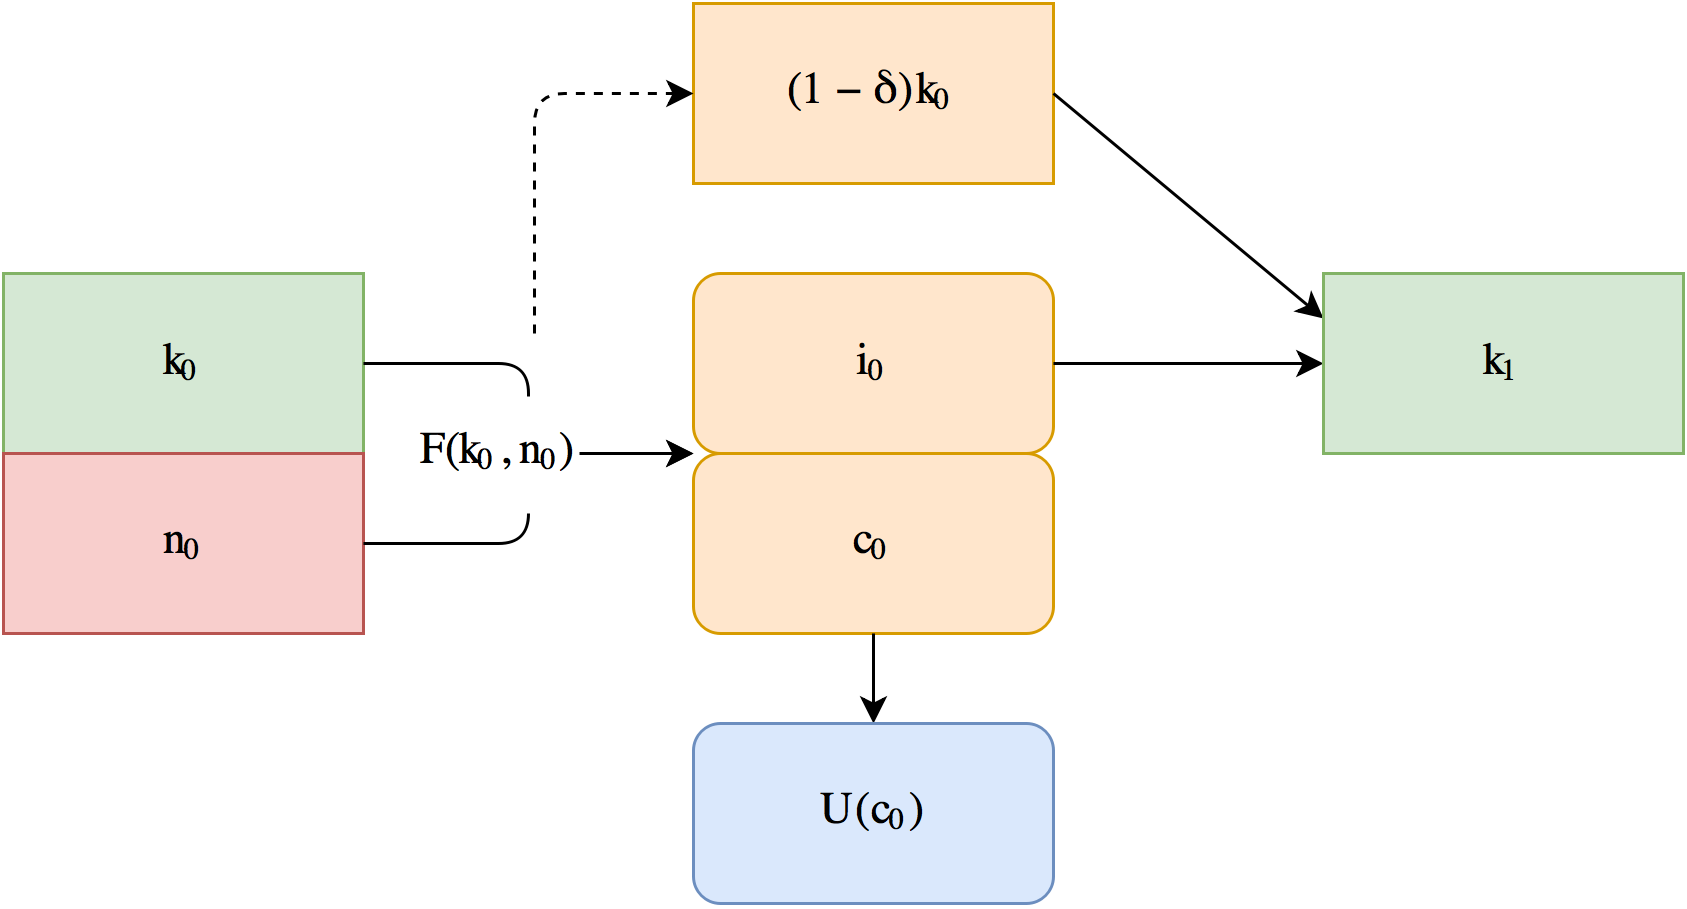
\includegraphics[width=350px]{01-growth1.png}
		\end{center} 



\section{Setup}

Let's make some assumptions about the production function. First, it will be continuously differentiable, strictly increasing, homogeneous of degree one, and strictly quasi-concave. Thus, we have constant returns to scale; and strict quasi-concavity suggests at unique solutions, although we are not quite there yet. Furthermore, we assume the following:
\begin{itemize}
	\itemsep0em
	\item $F(0,n)=0$,
	\item $F_k(k,n)>0$,
	\item $F_n(k,n) >0$
	\item $\lim_{k \rightarrow 0} F_k(k,1) = \infty$,
	\item $\lim_{k \rightarrow \infty} F_k(k,1) = 0$.
\end{itemize}
The first three bullets are straightforward enough. You can't produce anything without using capital; and using more capital and more labor imply more is produced.

The last two bullets are a little more troublesome in interpretation. The first limit says that if you using practically no capital, then increasing your use of capital has \emph{huge} returns in terms of output. The second limit says that if you're already using a lot of capital, then increasing your use of capital will have practically no effect on output. This collection of assumptions are known as the \textbf{Inada conditions}. Note that a Cobb-Douglas function satisfies the Inada conditions, hence its common usage in growth economics.

Now beyond the production function itself, let's suppose that the size of the population is constant over time. Recall that the labor force must satisfy $0 \leq n_t \leq 1$. 

Recall that the amount of capital in the next period can be written as 
	\[k_{t+1} = (1 - \delta)k_t + i_t \Lindent i_t = k_{t+1} - (1 - \delta)k_t.\]
Since today's output can be used for either today's consumption or today's investment, we can thus rewrite $c_t + i_t \leq y_t$ as 
	\[c_t + k_{t+1} - (1 - \delta)k_t \leq F(k_t, n_t).	\]	

We assume that all households have identical preferences over intertemporal consumption sequences, which again have the additively separable form 
	\[	\sum_{t=0}^{\infty} \beta^t U(c_t).\]
We will assume that $u(\cdot)$ is bounded, continuously differentiable, strictly increasing, strictly concave, and exhibits infinite marginal utility at consumption approaches zero. (Also notice that leisure is not valued -- great assumption! All work and no play makes Jack an economic theorist.) 


\section{Social Planner}

Let's take the perspective of a benevolent social planner who wants to maximize the sum of utilities by choosing sequences $\{(c_t, k_{t+1}, n_t) \}_{t=1}^{\infty}$. In other words, the social planner wants to choose how much to consume in each period, how much capital to have in each subsequent period, and how much people should work in each period, such that the choice maximizes the sum of (discounted) utilities over an infinite number of periods. Quite a task, no?

First, it should be clear that no output will actually be wasted. Consuming what would have been wasted output increases utility today; investing it will lead to increased possibility of consumption later, and thus higher utility later. So we can write as an equality
	\[c_t + k_{t+1} - (1 - \delta)k_t = F(k_t, n_t).	\]
Second, since leisure is not valued and the marginal product of labor is always positive, people will work full-time, that is, $n_t=1$. This will allow for more output, and thus more consumption, and thus more utility. 

One of the nice things about having $n_t=1$ is that $k_t$ and $y_t$ represent both total and per-capita capital and output. This allows us to write
	\[f(k_t) = F(k_t,1) + (1 - \delta)k_t\]
as the total supply of goods available per worker -- it is the amount of capital produced plus undepreciated capital. Think of it like this. The production process uses the $k_t$ capital, giving $F(k_t,1)$ output. In the production process, some of that capital breaks down, and we have $(1 - \delta)k_t$ capital left over. Thus, the total amount of the good available  is the output plus whatever hasn't broken down in the production process.

Many properties of $F(\cdot)$ are inherited by $f(\cdot)$. In particular, we can say the following about $f(\cdot)$: 
\begin{itemize}
	\itemsep0em
	\item Continuously differentiable
	\item Strictly increasing
	\item Strictly concave
	\item $f(0)=0$
	\item $f'(k) >0$
	\item $\lim_{k \rightarrow 0} f'(k)=\infty$
	\item $\lim_{k \rightarrow \infty} f'(k)=1 - \delta$.
\end{itemize}
The proof for each bullet point is pretty straightforward but feel free to do them as an exercise.


We can re-write the goods-per-worker equation as 
	\[f(k_t) - (1 - \delta)k_t = F(k_t,1).\]
Since we determined that there will be no wasted goods, and also determined that $n_t=1$, we also have the constraint 
	\[c_t + k_{t+1} - (1 - \delta)k_t = F(k_t, 1).\]
We can equate the left-hand side of both and then solve for consumption to get
	\[c_t =  f(k_t) - k_{t + 1} \Lindent 0 \leq k_{t+1} \leq f(k_t).	\]
Therefore we can write the social planner's problem as
\begin{align}
	\max_{ \{k_{t+1} \}_{t =0}^{\infty} } &\sum_{t = 0}^{\infty} \beta^t U\big( f(k_t) - k_{t + 1} \big) \label{spobjective}\\
	\text{ s.t. } \;\; &0 \leq k_{t+1} \leq f(k_t) \label{spcond}\\
	\text{ given} \;\; &k_0 > 0.
\end{align}
In other words, the planner wants to decide how much capital to have remaining in the next period in such a way as to maximize the sum of discounted utility. This in effect also decides how much is consumed in each period. 
		\begin{center}
			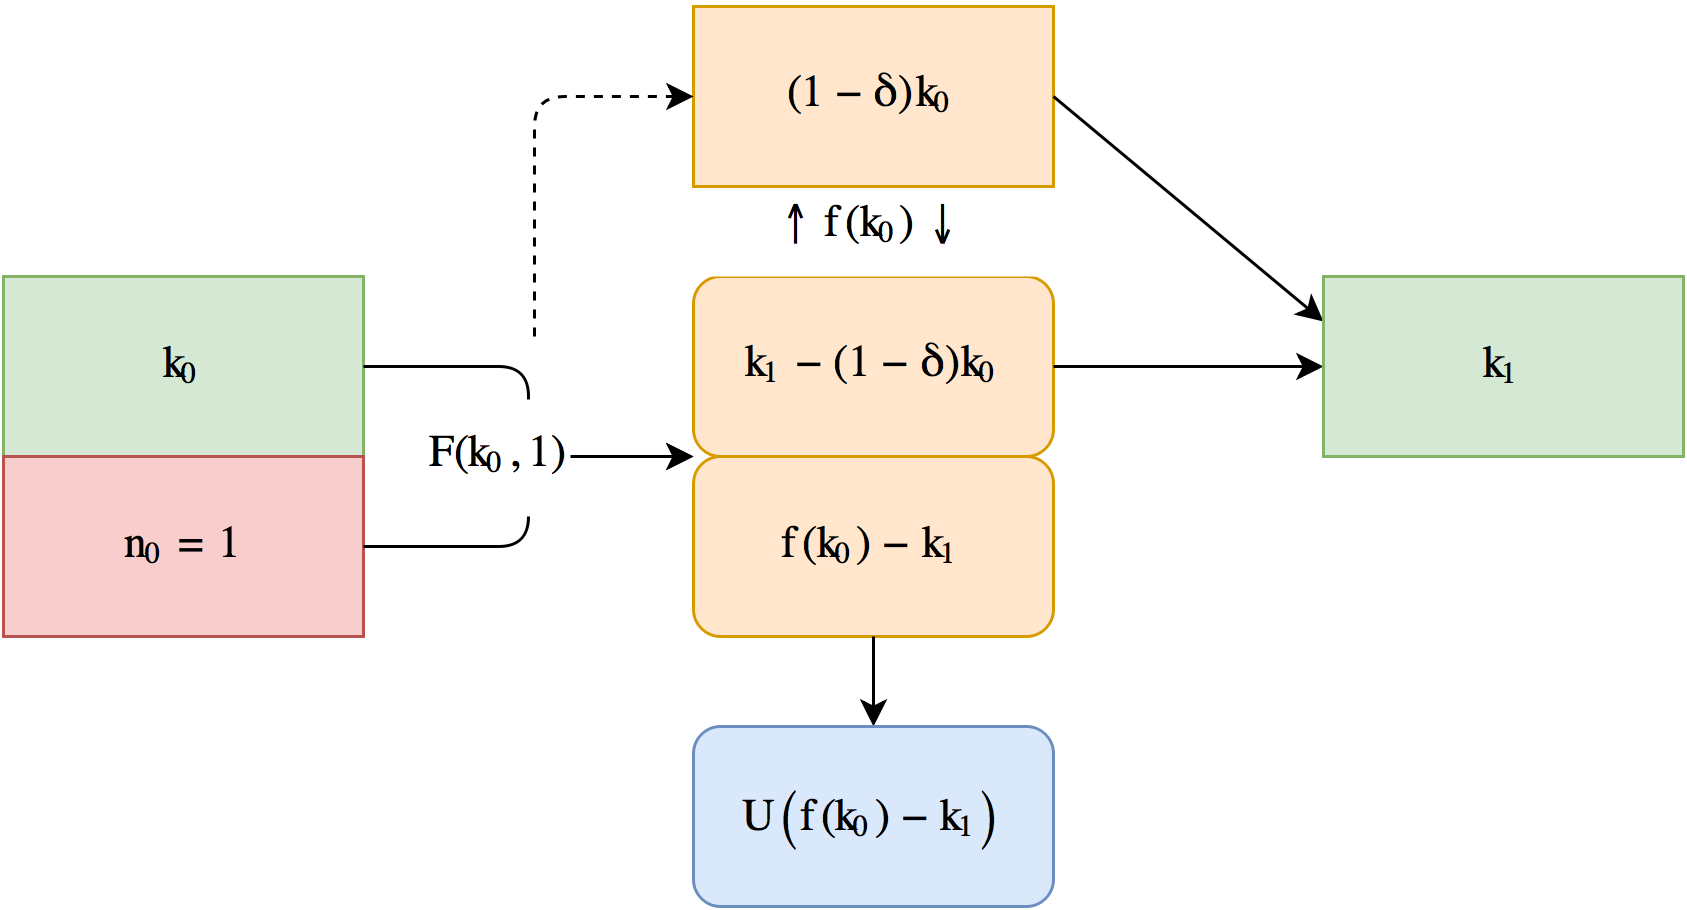
\includegraphics[width=350px]{01-growth2.png}
			
\small	The boxes in orange represent $f(k_0)$.
		\end{center} 

\subsection{Finite Horizon} 

Ultimately we are interested in the infinite horizon case, but it will be easier to first deal with a finite case. So suppose there are $T$ periods. 
The set of sequences satisfying equation (\ref{spcond}) will be closed, bounded, and convex. Furthermore, the objective function in (\ref{spobjective}) will be continuous and strictly concave. So the typical Kuhn-Tucker conditions will completely characterize the solution. That's nice. 

First of all, notice that the inequality constraints will only be binding in the final period -- there is no incentive to invest in the next period if you're gonna be dead. Thus, $k_{T+1}=0$. Consume everything in the final period! After all, the pre-apocalypse party \emph{should} be the party to end all parties. Thus, we have two \textbf{boundary conditions},
\begin{equation}
	k_{T+1}=0, \;\; k_0 >0.  \label{finitebc}
\end{equation}	
	
The first-order condition is simply the derivative of the sum of discounted utilities with respect to each $k+1$ in search of the critical point. Here's what I mean by that. Consider the first two terms in the utility sum,
	\[U\big( f(k_0) - k_{1} \big)	 + \beta U\big( f(k_1) - k_{2} \big) + ... \]
There are the only two terms that will contain $k_1$, which is what we are choosing apropos maximization in period 0. Thus, the derivative with respect to $k_1$, set equal to zero apropos a critical point, is 
	\[	
	-U'_{k_1}\big( f(k_0) - k_1 \big) 	+ \beta U'_{f(k_1)}\big( f(k_1) - k_2 \big)f'_{k_1}(k_1) :=0.
	\]
More generally, we'll have 
\begin{equation}
	 \beta U'_{f(k_t)}\big( f(k_t) - k_{t+1} \big) f'_{k_t}(k_t) = U'_{k_t} \big( f(k_{t-1}) - k_t \big) , \;\; t=1, ..., T. \label{finitefoc}
\end{equation}
Equation (\ref{finitefoc}) is a second order difference equation in $k_t$. For those with exposure to difference equations, this means it has a two-parameter family of solutions. The solution we're interested in is the one that also satisfies the boundary conditions. 



\section{Finite Horizon Example: Cobb-Douglas}

Let's consider a Cobb-Douglas production function. Since labor has been normalized to 1, the function is simply $f(k)=k^{\alpha}$. And let $U(c)=\ln(c)$. These should be pretty easy to work with, no? (Granted, this actually doesn't fit all of our assumptions. Perhaps this means the assumptions are sufficient but not necessary...?)

What we're aiming to solve is 
\begin{align}
	\max_{ \{k_{t+1} \}_{t =0}^{\infty} } &\sum_{t = 0}^{\infty} \beta^t \ln\big( k_t^{\alpha} - k_{t + 1} \big) \label{spobjective}\\
	\text{ s.t. } \;\; &0 \leq k_{t+1} \leq k_t^{\alpha}, \label{spcond}\\
		&k_{T+1}=0,\\
	\text{ given} \;\; &k_0 > 0.
\end{align}


\subsection{Fixed Points}

The first-order condition, after a little bit of rearranging, is
	\[\frac{k_t}{k_{t-1}^{\alpha} - k_t}= \alpha \beta \frac{ k_t^{\alpha}}{k_t^{\alpha} - k_{t+1}}.	\]
Let $z_t = k_t / k_{t - 1}^{\alpha}$, noting that $z_{t+1} = k_{t+1} / k_{t }^{\alpha}$. Perform the following multiplications,
	\[ \left(\frac{ 1 / k^{\alpha}_{t - 1}}{1 / k^{\alpha}_{t - 1}}\right) \frac{k_t}{k_{t-1}^{\alpha} - k_t}= \alpha \beta \frac{ k_t^{\alpha}}{k_t^{\alpha} - k_{t+1}} \left( \frac{1/k_{t + 1}}{1 / k_{t + 1}}\right),	\]
	to get the first-order difference equation in $z_t$, 
	\[
		\frac{z_t}{1 -z_t} = \alpha \beta \frac{  1}{1- z_{t+1}},
	\]
which we can explicitly solve for $z_{t+1}$:
\begin{equation}
	z_{t + 1} = 1 + \alpha \beta - \frac{\alpha \beta}{z_t}. \label{finiteexzt}
\end{equation}

If you plot the $45^{\circ}$ line and start from some initial $z_t$,  you will (probably) find yourself gravitating closer and closer to a certain point. In particular, the point $z_t=1$. Indeed, if you plug $z_t=1$ into equation (\ref{finiteexzt}), you will get $z_{t+1}=1$. Turns out that $z_t=1$ is a \textbf{fixed point}, which indicates a \textbf{steady state}. (You might notice that $z_t=\alpha \beta$ is also a fixed point -- hence the ``probably'' a few sentences ago. This is the bad steady-state. I'll neglect it for now.) This means that the fixed point satisfies $ k_t =  k_{t - 1}^a = f(k_{t-1})$. In other words, the economy in its (good) steady-state seems to have a fixed ``rule'' by which it determines how much capital to carry over to the next period. Keep that suggestion tucked in the back of your mind. 


\subsection{Solving for \bm{$z_t$}}

Okay, so that's a nice result. It would be nicer if we had a closed form solution for $z_t$, however. Turns out we can find one by using the boundary condition. Since $k_{T+1}=0$, it follows that $z_{T+0} = 0$. Shoving this into equation (\ref{finiteexzt}), we end up with
	\[	z_T = \alpha \beta\frac{1}{1 + \alpha \beta}.\]
And then shoving this into  equation (\ref{finiteexzt}), we end up with
	\[ z_{T - 1} = \alpha \beta \frac{ 1 + \alpha \beta}{1 + \alpha \beta + (\alpha\beta)^2} .\]
Okay, one more time. Shove this into  equation (\ref{finiteexzt}) again to get
	\[z_{T-2} = \alpha \beta \frac{1 + \alpha \beta + (\alpha \beta)^2}{1 + \alpha \beta + (\alpha\beta)^2 + (\alpha\beta)^3}.	\]
Hopefully you see the pattern by now and we can generalize this to
	\[z_{T-j} = \alpha \beta \frac{ \sum_{i=0}^j (\alpha \beta)^j}{ \sum_{i=0}^j (\alpha \beta)^{j+1}}. \]
Finally, just to make the equation as straightforward as possible, have $t=T-j$ so $j = T-t$. Then we can write
	\[ z_t =  \alpha \beta \frac{ \sum_{i=0}^j (\alpha \beta)^{T-t}}{ \sum_{i=0}^j (\alpha \beta)^{T-t+1}}.	\label{cdcfsums}\]

This is indeed a closed form solution, but it's still not very user-friendly. In particular, having a bunch of sums is no fun. But we know some tricks apropos evaluating sums. Consider the sum in the numerator -- call it $S_{T-t}$. That is,
	\[S_{T-t} =  \sum_{i=0}^j (\alpha \beta)^{T-t} .\]
Now multiply both sides by $\alpha \beta$ and we have
	\[\alpha \beta S_{T-t} =  \sum_{i=0}^j (\alpha \beta)^{T-t+1} .\]
Subtract the two (write out each term in the sum explicitly if you have to) to get
	\[ S_{T-t} - \alpha \beta S_{T-t} = 1 - (\alpha \beta)^{T -t +1}.\]
Thus, solving for $S_{T-t}$, we have
	\[	S_{T-t}	= \frac{ 1 - (\alpha \beta)^{T -t +1}}{1 - \alpha \beta}. \]
The denominator would be similar except the index would be one greater. Thus, we can plug the two sums into equation (\ref{cdcfsums}), canceling out the common denominators, to get the rather elegant form
\begin{equation}
	z_t = \alpha \beta \frac{ 1 - (\alpha \beta)^{T -t +1}}{ 1 - (\alpha \beta)^{T -t +2}}.	 \label{cdztsol}
\end{equation}


\subsection{Solving for \bm{$k_{t+1}$}}

We have defined $z_t = k_t / k^{\alpha}_{t-1}$.  Thus we can write equation (\ref{cdztsol}) as 
\begin{equation}
	\frac{k_t}{k^{\alpha}_{t-1}} = 	\alpha \beta\frac{ 1 - (\alpha \beta)^{T -t +1}}{ 1 - (\alpha \beta)^{T -t +2}} \Lindent k_t = \alpha \beta \frac{ 1 - (\alpha \beta)^{T -t +1}}{ 1 - (\alpha \beta)^{T -t +2}}k^{\alpha}_{t-1}. \label{cdlomoc} 
\end{equation}
Equation (\ref{cdlomoc}) defines the \textbf{law of motion of capital}. It might be worth verifying that this equation satisfies the first-order conditions. Recall that we must have
	\[\frac{k_t}{k_{t-1}^{\alpha} - k_t}= \alpha \beta \frac{ k_t^{\alpha}}{k_t^{\alpha} - k_{t+1}}	\]
as the first-order condition.

Let's first analyze the left-hand side. Plugging in the closed form solutions for $k_t$, and $k_{t+1}$, we have the quite messy
	\[LHS = \dfrac{ \alpha \beta \dfrac{ 1 - (\alpha \beta)^{T -t +1}}{ 1 - (\alpha \beta)^{T -t +2}}k^{\alpha}_{t-1}}{k_{t-1}^{\alpha} -  \alpha \beta\dfrac{ 1 - (\alpha \beta)^{T -t +1}}{ 1 - (\alpha \beta)^{T -t +2}}k^{\alpha}_{t-1}}.\]
For clarity's sake, define 
	\[ \sigma = \alpha \beta \frac{ 1 - (\alpha \beta)^{T -t +1}}{ 1 - (\alpha \beta)^{T -t +2}} \Lindent LHS = \frac{ \sigma k^{\alpha}_{t-1}}{k_{t-1}^{\alpha} -  \sigma k^{\alpha}_{t-1}} = \frac{\sigma}{1 - \sigma}.\]
This is much more elegant in appearance.

Now let's analyze the right-hand side. Again substituting in the closed forms for $k_t$ and $k_{t+1}$, and doing some cancellations, we have
	\[	RHS = \alpha \beta \frac{1}{1 - \alpha \beta \frac{ 1 - (\alpha \beta)^{T -t}}{ 1 - (\alpha \beta)^{T -t +1}}} = \alpha \beta \frac{1 - (\alpha \beta)t^{T -t +1}}{ 1 - \alpha \beta}.	\]
Multiply numerator and denominator by 
\[	RHS =  \alpha \beta \frac{1 - (\alpha \beta)^{T -t +1}}{ 1 - \alpha \beta} \left( \frac{ 1 - (\alpha \beta)^{T -t +2}}{ 1 - (\alpha \beta)^{T -t +2}} \right) = \sigma \frac{ 1 - (\alpha \beta)^{T -t +2}}{1 - \alpha \beta}.	\]
Now just notice that 
	\[ \frac{1}{1 - \sigma} =   \frac{   1 - (\alpha \beta)^{T -t +2} }{ 1 - \alpha \beta} \Lindent RHS= \frac{\sigma}{1- \sigma}.	\]
Great, so the LHS and the RHS are equal and we can confirm that this law of motion of capital satisfies the first-order condition.

Finally, let's make sure the relevant boundary condition holds:
\[	 k_{T+1} = \alpha \beta \frac{ 1 - (\alpha \beta)^{0}}{ 1 - (\alpha \beta)^{1}}k^{\alpha}_{T} =0. \]
Cool, both the first-order condition and the boundary condition holds, so we can confirm that the law of motion of capital we've found is optimal. 


\end{document}
 